\documentclass{article}
\usepackage{graphicx}
\usepackage{amsmath}
\usepackage{amssymb}
\usepackage{array}
\providecommand{\cbrak}[1]{\ensuremath{\left\{#1\right\}}}

\begin{document}
\begin{enumerate}

\item The graph of $y = p(x)$ is shown in Figure 1 for some polynomial $p(x)$. Find the number of zeroes of $p(x)$.

\begin{figure}[h]
\centering
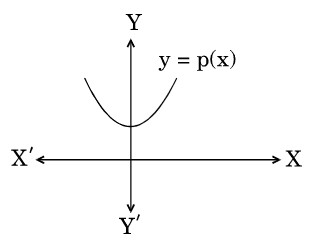
\includegraphics[width=0.4\columnwidth]{ques8.jpg}
\caption{}
\end{figure}

\item If $f(x) = \frac{1-x}{1+x}$, then find $(f\circ f)(x)$.


\item Let $W$ denote the set of words in the English dictionary. Define the relation $R$ by
$R$ = $\cbrak{(x, y) \in W \times W \mid} x$ and $y$ have at least one letter in common.
Show that this relation $R$ is reflexive and symmetric, but not transitive.
\item Find the inverse of the function $f(x) = (\frac{4x}{3x+4})$.

\item The value of $k(k < 0)$ for which the function $f$ defined as 
\begin{align*}
f(x) = \begin{cases}
x^2, & \text{if } x < 0 \\
\sin(x), & \text{if } x \geq 0  \\
\end{cases}
\end{align*}
is continuous at $x = 0$ is:

\begin{enumerate}
     \item $\pm1$ 

     \item $\pm1$ 

     \item  $\pm\frac{1}{2}$ 

     \item  $\frac{1}{2}$ 

\end{enumerate}


\item Find the intervals in which the function $f$ given by $f(x) = x^2 – 4x + 6$ is strictly
increasing:

\begin{enumerate}

     \item $(-\infty,2) \bigcup (2,\infty)$ 
     
     \item $(2,\infty)$ 

     \item $(-\infty,2)$ 

     \item $(-\infty,2) \bigcup (2,\infty)$ 
\end{enumerate}


\newpage

\item The real function $f(x) = 2x3 – 3x2 – 36x + 7$ is:

\begin{enumerate}

     \item Strictly increasing in $(-\infty,-2)$ and strictly decreasing in $(-2,\infty)$
     
     \item Strictly decreasing in $(-2,3)$ 

     \item Strictly decreasing in $(-\infty,3)$ and strictly increasing in $(3,\infty)$ 

     \item Strictly decreasing in $(-\infty,2) \bigcup (3,\infty)$

\end{enumerate}


\item The value of $b$  for which the function $f(x) = x + cosx + b$ is strictly decreasing over \textbf{R} is:
\begin{enumerate}

     \item $b < 1$ 
     
     \item No value of $b$ exists 

     \item $b \leq 1$ 

     \item $b \geq 1$ 

\end{enumerate}

\item The point(s), at which the function $f$ given by  

\begin{align*}
f(x) = \begin{cases}
\frac{x}{|x|}, x < 0 \\
-1 , x \geq 0 \\
\end{cases}
\end{align*}
is continuous, is/are:
\begin{enumerate}
     \item $x\varepsilon R$ 
     \item $x = 0$
     \item $x\varepsilon R -\{0\}$ 
     \item $x = -1$ and $1$ 
\end{enumerate}

\item The area of a trapezium is defined by function $f$ and given by $f(x) = (10 + x)\sqrt{100-x^2}$
, then the area when it is maximised is: 
\begin{enumerate}
    \item $75cm^2$
    \item $7\sqrt{3}cm^2$
    \item $75\sqrt{3}cm^2$
    \item $5cm^2$
\end{enumerate}

\item If $tan^{-1} x = y$, then: 
\begin{enumerate}
    \item $-1 < y < 1$
    \item $\frac{-\pi}{2} \leq y \leq \frac{\pi}{2}$
    \item $\frac{-\pi}{2} < y < \frac{\pi}{2}$
    \item $y \varepsilon\{\frac{-\pi}{2},\frac{\pi}{2}\}$
\end{enumerate}


\end{enumerate}

\end{document}
